\subsection{Components}

\begin{figure}
  \centering
    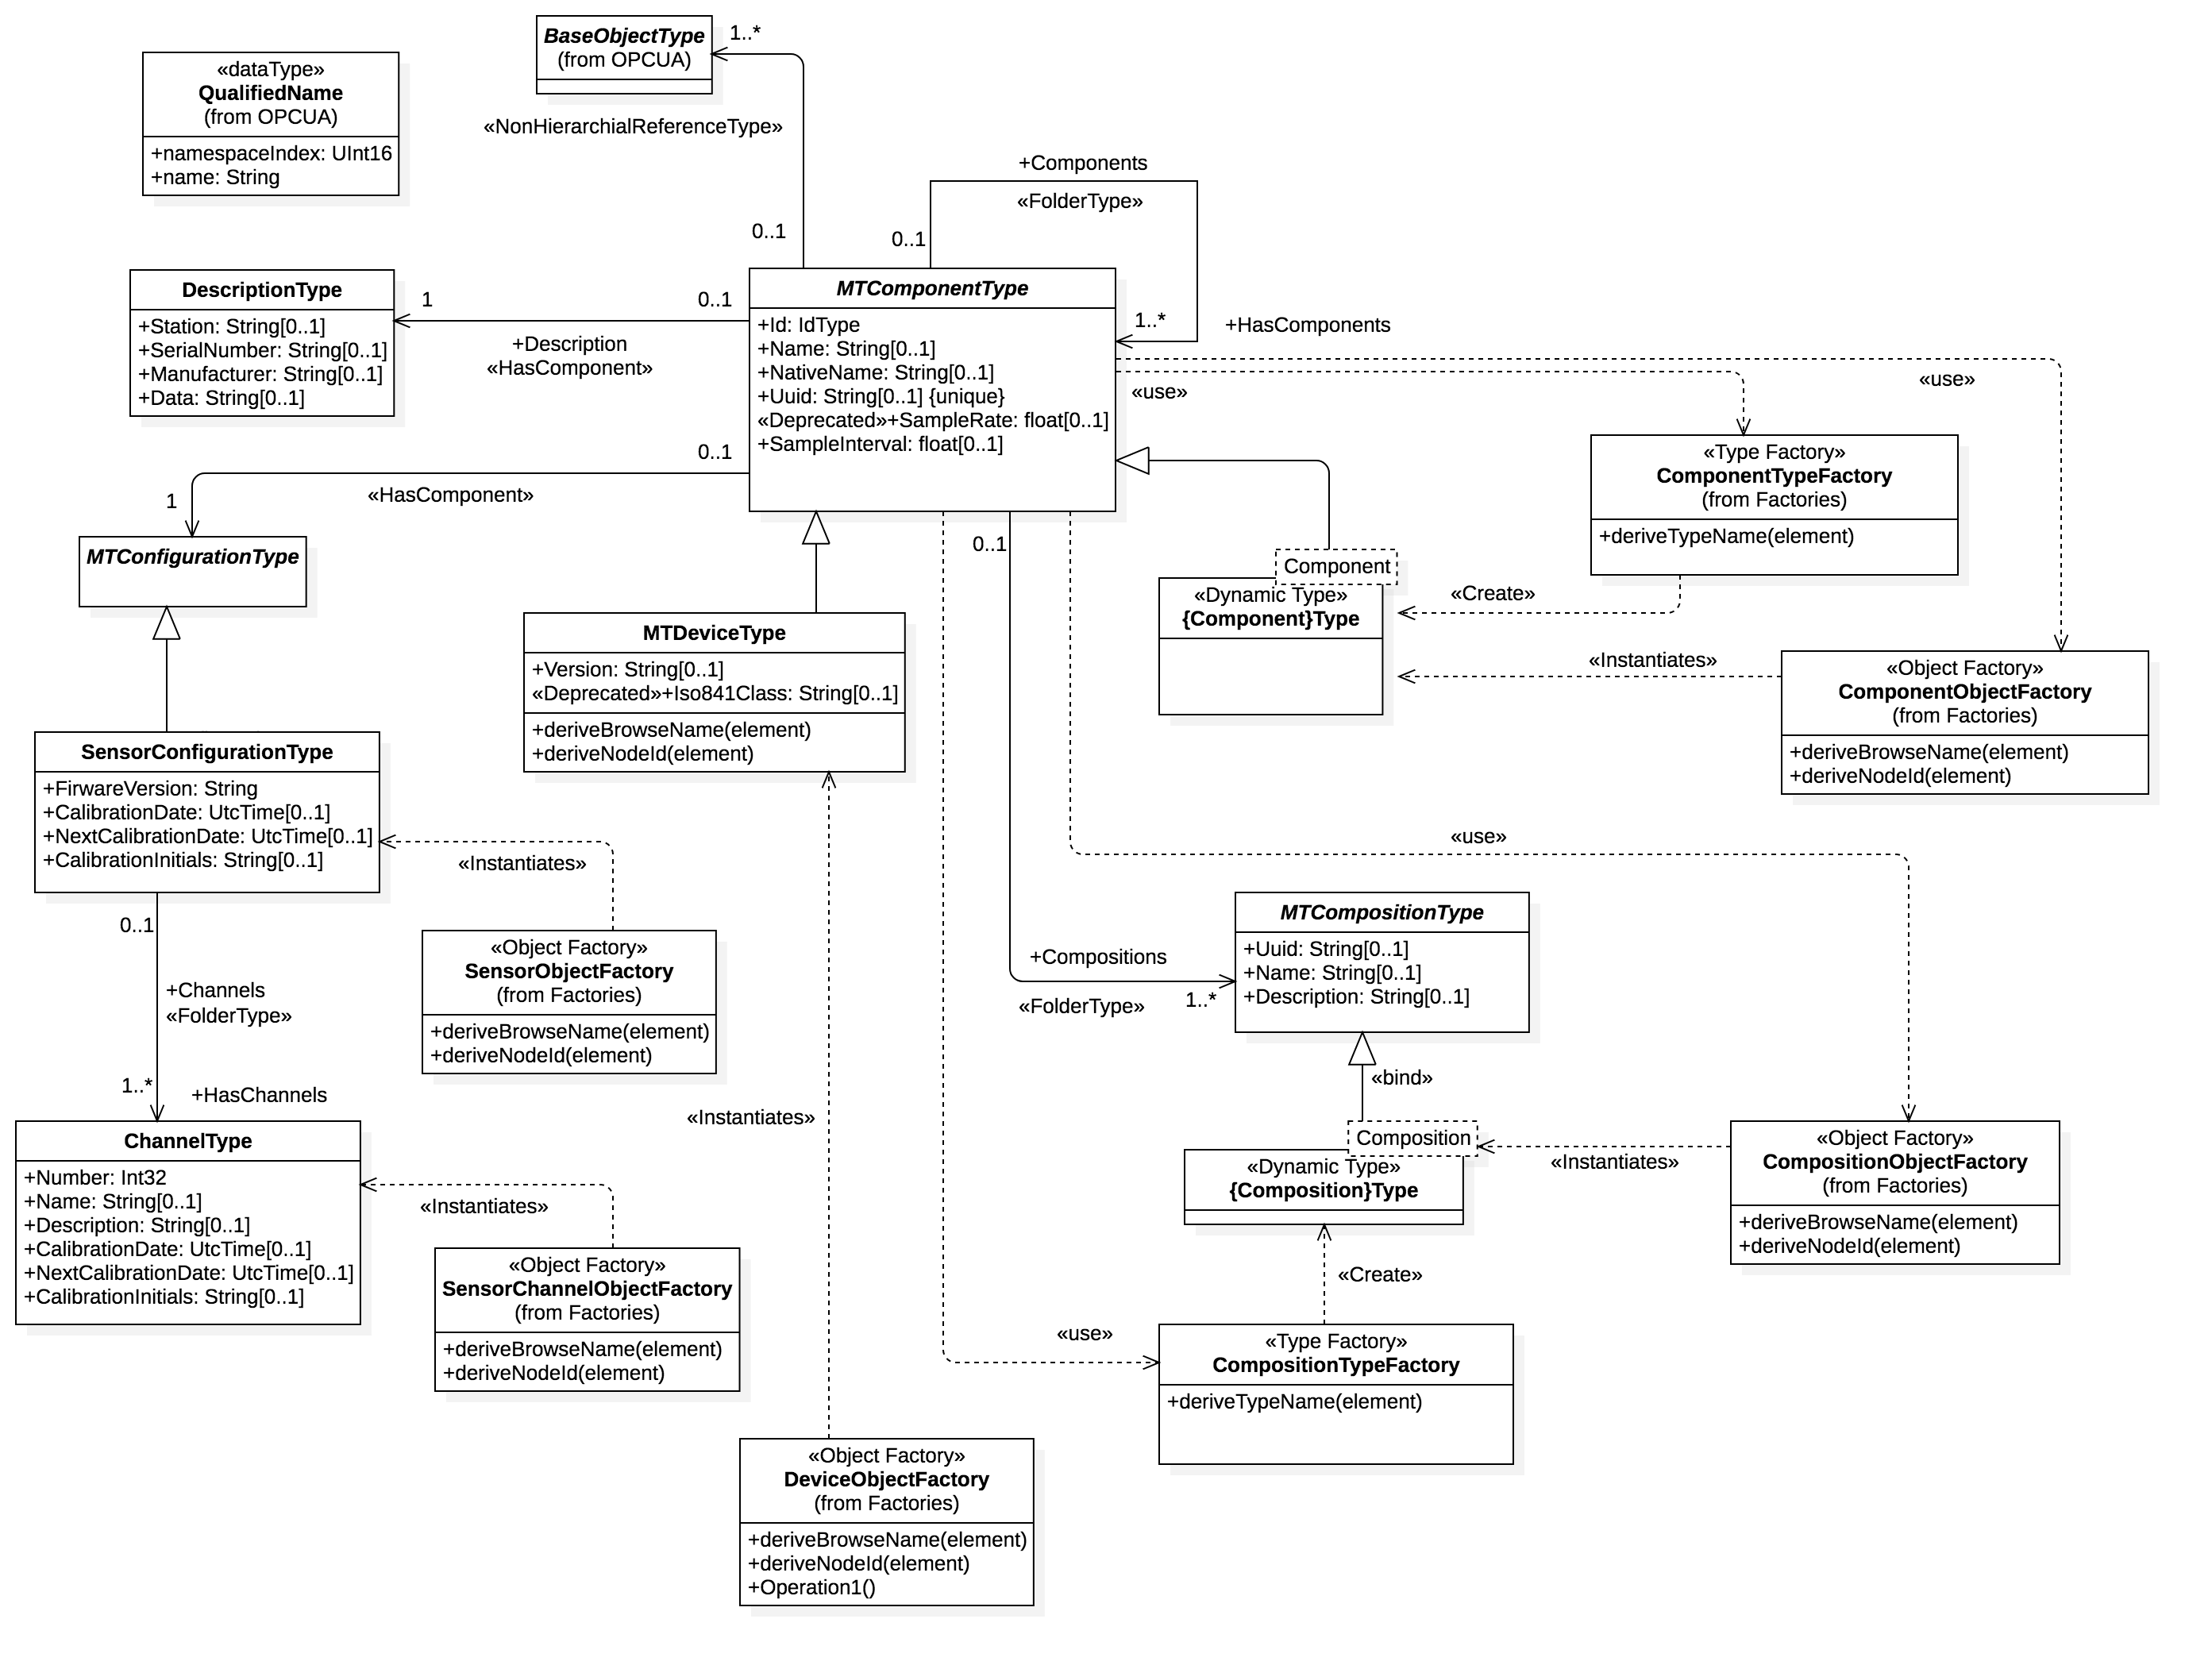
\includegraphics[width=1.0\textwidth]{diagrams/Components.png}
  \caption{Components Diagram}
  \label{fig:Components}
\end{figure}


The Components documents the Component models and the owned objects.

\subsubsection{Defintion of ChannelType} \label{type:ChannelType}



Refer to Table \ref{table:ChannelType} for detailed definition.

\begin{table}
\centering 
  \caption{ChannelType Definition}
  \label{table:ChannelType}
\footnotesize
\tabulinesep=3pt
\begin{tabu} to 6in {|X[1.3]|X[1]|X[1.6]|X[2]|X[1.5]|X[1]|} \everyrow{\hline}
\hline
\rowfont\bfseries {Attribute} & \multicolumn{5}{|l|}{Value} \\
\tabucline[1.5pt]{}
BrowseName & \multicolumn{5}{|l|}{ChannelType} \\
IsAbstract & \multicolumn{5}{|l|}{False} \\
\tabucline[1.5pt]{}
\rowfont \bfseries References & NodeClass & BrowseName & DataType & TypeDefinition & {Modeling Rule} \\
\multicolumn{6}{|l|}{Subtype of BaseObjectType (See OPCUA Documentation)} \\
HasProperty & Variable & Number &  Int32 & PropertyType & Manditory \\
HasProperty & Variable & Name &  String & PropertyType & Optional \\
HasProperty & Variable & Description &  String & PropertyType & Optional \\
HasProperty & Variable & CalibrationDate &  UtcTime & PropertyType & Optional \\
HasProperty & Variable & NextCalibrationDate &  UtcTime & PropertyType & Optional \\
HasProperty & Variable & CalibrationInitials &  String & PropertyType & Optional \\
\end{tabu}
\end{table} 

\subsubsection{Defintion of DescriptionType} \label{type:DescriptionType}

Exact mirror of the MTConnect Type.

Refer to Table \ref{table:DescriptionType} for detailed definition.

\begin{table}
\centering 
  \caption{DescriptionType Definition}
  \label{table:DescriptionType}
\footnotesize
\tabulinesep=3pt
\begin{tabu} to 6in {|X[1.3]|X[1]|X[1.6]|X[2]|X[1.5]|X[1]|} \everyrow{\hline}
\hline
\rowfont\bfseries {Attribute} & \multicolumn{5}{|l|}{Value} \\
\tabucline[1.5pt]{}
BrowseName & \multicolumn{5}{|l|}{DescriptionType} \\
IsAbstract & \multicolumn{5}{|l|}{False} \\
\tabucline[1.5pt]{}
\rowfont \bfseries References & NodeClass & BrowseName & DataType & TypeDefinition & {Modeling Rule} \\
\multicolumn{6}{|l|}{Subtype of BaseObjectType (See OPCUA Documentation)} \\
HasProperty & Variable & Station &  String & PropertyType & Optional \\
HasProperty & Variable & SerialNumber &  String & PropertyType & Optional \\
HasProperty & Variable & Manufacturer &  String & PropertyType & Optional \\
HasProperty & Variable & Data &  String & PropertyType & Optional \\
\end{tabu}
\end{table} 

\subsubsection{Defintion of MTComponentType} \label{type:MTComponentType}

The base Component Type from which all MTConnect Components are derived from. The 
component type factory is used to create the specific OPC/UA types as subtypes of the 
MTConnect `MTComponentType`. The component types will be created once for all Component objects 
of that type based on the `QName` of the MTConnect XML element. 

The object factory will instantiate the Component Objects and insert them into the Components 
folder with a browse name of the Component QName and the `name` element if specified surrounded 
by square brackets, `[]`. For example if the MTConnect Element is:

`<Linear name='X'>...</...>`

The OPC/UA Object with browse name `Linear[X]` will be created with the HasTypeDefinition 
referencing the `Linear` OPC/UA type. 

The meta data for the component and it's relationships are static. The dynamic data will be 
represented using the _OPC/UA Part 8_ 



Refer to Table \ref{table:MTComponentType} for detailed definition.

\begin{table}
\centering 
  \caption{MTComponentType Definition}
  \label{table:MTComponentType}
\footnotesize
\tabulinesep=3pt
\begin{tabu} to 6in {|X[1.3]|X[1]|X[1.6]|X[2]|X[1.5]|X[1]|} \everyrow{\hline}
\hline
\rowfont\bfseries {Attribute} & \multicolumn{5}{|l|}{Value} \\
\tabucline[1.5pt]{}
BrowseName & \multicolumn{5}{|l|}{MTComponentType} \\
IsAbstract & \multicolumn{5}{|l|}{True} \\
\tabucline[1.5pt]{}
\rowfont \bfseries References & NodeClass & BrowseName & DataType & TypeDefinition & {Modeling Rule} \\
HasProperty & Variable & Id &  IdType & PropertyType & Manditory \\
HasProperty & Variable & Name &  String & PropertyType & Optional \\
HasProperty & Variable & NativeName &  String & PropertyType & Optional \\
HasProperty & Variable & Uuid &  String & PropertyType & Optional \\
HasProperty & Variable & SampleRate &  float & PropertyType & Optional \\
HasProperty & Variable & SampleInterval &  float & PropertyType & Optional \\
HasComponent & Object & Description &   & DescriptionType & Optional \\
HasComponent & Object & Configuration &   & MTConfigurationType & Optional \\
Organizes & Object & Components &  MTComponentType & FolderType & Optional \\
Organizes & Object & Compositions &  MTCompositionType & FolderType & Optional \\
HasProperty & Variable & <Dynamic> &  {DataItem}Type & <Dynamic> & Optional \\
HasProperty & Variable & <Dynamic> &  BaseObjectType & <Dynamic> & Optional \\
Organizes & Object & Conditions &  MTNonExclusiveConditionType & FolderType & Optional \\
HasProperty & Variable & <Dynamic> &  {DataItem}Type & <Dynamic> & Manditory \\
\end{tabu}
\end{table} 

\subsubsection{Defintion of MTCompositionType} \label{type:MTCompositionType}



Refer to Table \ref{table:MTCompositionType} for detailed definition.

\begin{table}
\centering 
  \caption{MTCompositionType Definition}
  \label{table:MTCompositionType}
\footnotesize
\tabulinesep=3pt
\begin{tabu} to 6in {|X[1.3]|X[1]|X[1.6]|X[2]|X[1.5]|X[1]|} \everyrow{\hline}
\hline
\rowfont\bfseries {Attribute} & \multicolumn{5}{|l|}{Value} \\
\tabucline[1.5pt]{}
BrowseName & \multicolumn{5}{|l|}{MTCompositionType} \\
IsAbstract & \multicolumn{5}{|l|}{True} \\
\tabucline[1.5pt]{}
\rowfont \bfseries References & NodeClass & BrowseName & DataType & TypeDefinition & {Modeling Rule} \\
\multicolumn{6}{|l|}{Subtype of BaseObjectType (See OPCUA Documentation)} \\
HasProperty & Variable & Uuid &  String & PropertyType & Optional \\
HasProperty & Variable & Name &  String & PropertyType & Optional \\
HasProperty & Variable & Description &  String & PropertyType & Optional \\
NonHierarchialReferenceType & Object & composition &  {DataItem}Type & NonHierarchialReferenceType & Optional \\
\end{tabu}
\end{table} 

\subsubsection{Defintion of MTConfigurationType} \label{type:MTConfigurationType}



Refer to Table \ref{table:MTConfigurationType} for detailed definition.

\begin{table}
\centering 
  \caption{MTConfigurationType Definition}
  \label{table:MTConfigurationType}
\footnotesize
\tabulinesep=3pt
\begin{tabu} to 6in {|X[1.3]|X[1]|X[1.6]|X[2]|X[1.5]|X[1]|} \everyrow{\hline}
\hline
\rowfont\bfseries {Attribute} & \multicolumn{5}{|l|}{Value} \\
\tabucline[1.5pt]{}
BrowseName & \multicolumn{5}{|l|}{MTConfigurationType} \\
IsAbstract & \multicolumn{5}{|l|}{True} \\
\tabucline[1.5pt]{}
\rowfont \bfseries References & NodeClass & BrowseName & DataType & TypeDefinition & {Modeling Rule} \\
\multicolumn{6}{|l|}{Subtype of BaseObjectType (See OPCUA Documentation)} \\
\end{tabu}
\end{table} 

\subsubsection{Defintion of MTDeviceType} \label{type:MTDeviceType}

The MTDevice is a special type whose object will be the root of the device graph. The Device uses the component type factory and the component object factories to create each of the first level components. 

The  compositions, relationships, and data items are then recursively created as one decendes the MTConnect informaiton model.

Refer to Table \ref{table:MTDeviceType} for detailed definition.

\begin{table}
\centering 
  \caption{MTDeviceType Definition}
  \label{table:MTDeviceType}
\footnotesize
\tabulinesep=3pt
\begin{tabu} to 6in {|X[1.3]|X[1]|X[1.6]|X[2]|X[1.5]|X[1]|} \everyrow{\hline}
\hline
\rowfont\bfseries {Attribute} & \multicolumn{5}{|l|}{Value} \\
\tabucline[1.5pt]{}
BrowseName & \multicolumn{5}{|l|}{MTDeviceType} \\
IsAbstract & \multicolumn{5}{|l|}{False} \\
\tabucline[1.5pt]{}
\rowfont \bfseries References & NodeClass & BrowseName & DataType & TypeDefinition & {Modeling Rule} \\
\multicolumn{6}{|l|}{Subtype of MTComponentType (see section \ref{type:MTComponentType})} \\
HasProperty & Variable & Version &  String & PropertyType & Optional \\
HasProperty & Variable & Iso841Class &  String & PropertyType & Optional \\
\end{tabu}
\end{table} 

\subsubsection{Defintion of SensorConfigurationType} \label{type:SensorConfigurationType}

The SensorConfiguration browse name will be created as an Object relationship with the parent component.

Refer to Table \ref{table:SensorConfigurationType} for detailed definition.

\begin{table}
\centering 
  \caption{SensorConfigurationType Definition}
  \label{table:SensorConfigurationType}
\footnotesize
\tabulinesep=3pt
\begin{tabu} to 6in {|X[1.3]|X[1]|X[1.6]|X[2]|X[1.5]|X[1]|} \everyrow{\hline}
\hline
\rowfont\bfseries {Attribute} & \multicolumn{5}{|l|}{Value} \\
\tabucline[1.5pt]{}
BrowseName & \multicolumn{5}{|l|}{SensorConfigurationType} \\
IsAbstract & \multicolumn{5}{|l|}{False} \\
\tabucline[1.5pt]{}
\rowfont \bfseries References & NodeClass & BrowseName & DataType & TypeDefinition & {Modeling Rule} \\
\multicolumn{6}{|l|}{Subtype of MTConfigurationType (see section \ref{type:MTConfigurationType})} \\
HasProperty & Variable & FirwareVersion &  String & PropertyType & Manditory \\
HasProperty & Variable & CalibrationDate &  UtcTime & PropertyType & Optional \\
HasProperty & Variable & NextCalibrationDate &  UtcTime & PropertyType & Optional \\
HasProperty & Variable & CalibrationInitials &  String & PropertyType & Optional \\
Organizes & Object & Channels &  ChannelType & FolderType & Optional \\
\end{tabu}
\end{table} 

\subsubsection{Defintion of {Component}Type} \label{type:{Component}Type}



Refer to Table \ref{table:{Component}Type} for detailed definition.

\begin{table}
\centering 
  \caption{{Component}Type Definition}
  \label{table:{Component}Type}
\footnotesize
\tabulinesep=3pt
\begin{tabu} to 6in {|X[1.3]|X[1]|X[1.6]|X[2]|X[1.5]|X[1]|} \everyrow{\hline}
\hline
\rowfont\bfseries {Attribute} & \multicolumn{5}{|l|}{Value} \\
\tabucline[1.5pt]{}
BrowseName & \multicolumn{5}{|l|}{{Component}Type} \\
IsAbstract & \multicolumn{5}{|l|}{False} \\
\tabucline[1.5pt]{}
\rowfont \bfseries References & NodeClass & BrowseName & DataType & TypeDefinition & {Modeling Rule} \\
\multicolumn{6}{|l|}{Subtype of MTComponentType (see section \ref{type:MTComponentType})} \\
\end{tabu}
\end{table} 

\subsubsection{Defintion of {Composition}Type} \label{type:{Composition}Type}



Refer to Table \ref{table:{Composition}Type} for detailed definition.

\begin{table}
\centering 
  \caption{{Composition}Type Definition}
  \label{table:{Composition}Type}
\footnotesize
\tabulinesep=3pt
\begin{tabu} to 6in {|X[1.3]|X[1]|X[1.6]|X[2]|X[1.5]|X[1]|} \everyrow{\hline}
\hline
\rowfont\bfseries {Attribute} & \multicolumn{5}{|l|}{Value} \\
\tabucline[1.5pt]{}
BrowseName & \multicolumn{5}{|l|}{{Composition}Type} \\
IsAbstract & \multicolumn{5}{|l|}{False} \\
\tabucline[1.5pt]{}
\rowfont \bfseries References & NodeClass & BrowseName & DataType & TypeDefinition & {Modeling Rule} \\
\multicolumn{6}{|l|}{Subtype of MTCompositionType (see section \ref{type:MTCompositionType})} \\
\end{tabu}
\end{table} 

\subsection{Data Items}

\begin{figure}
  \centering
    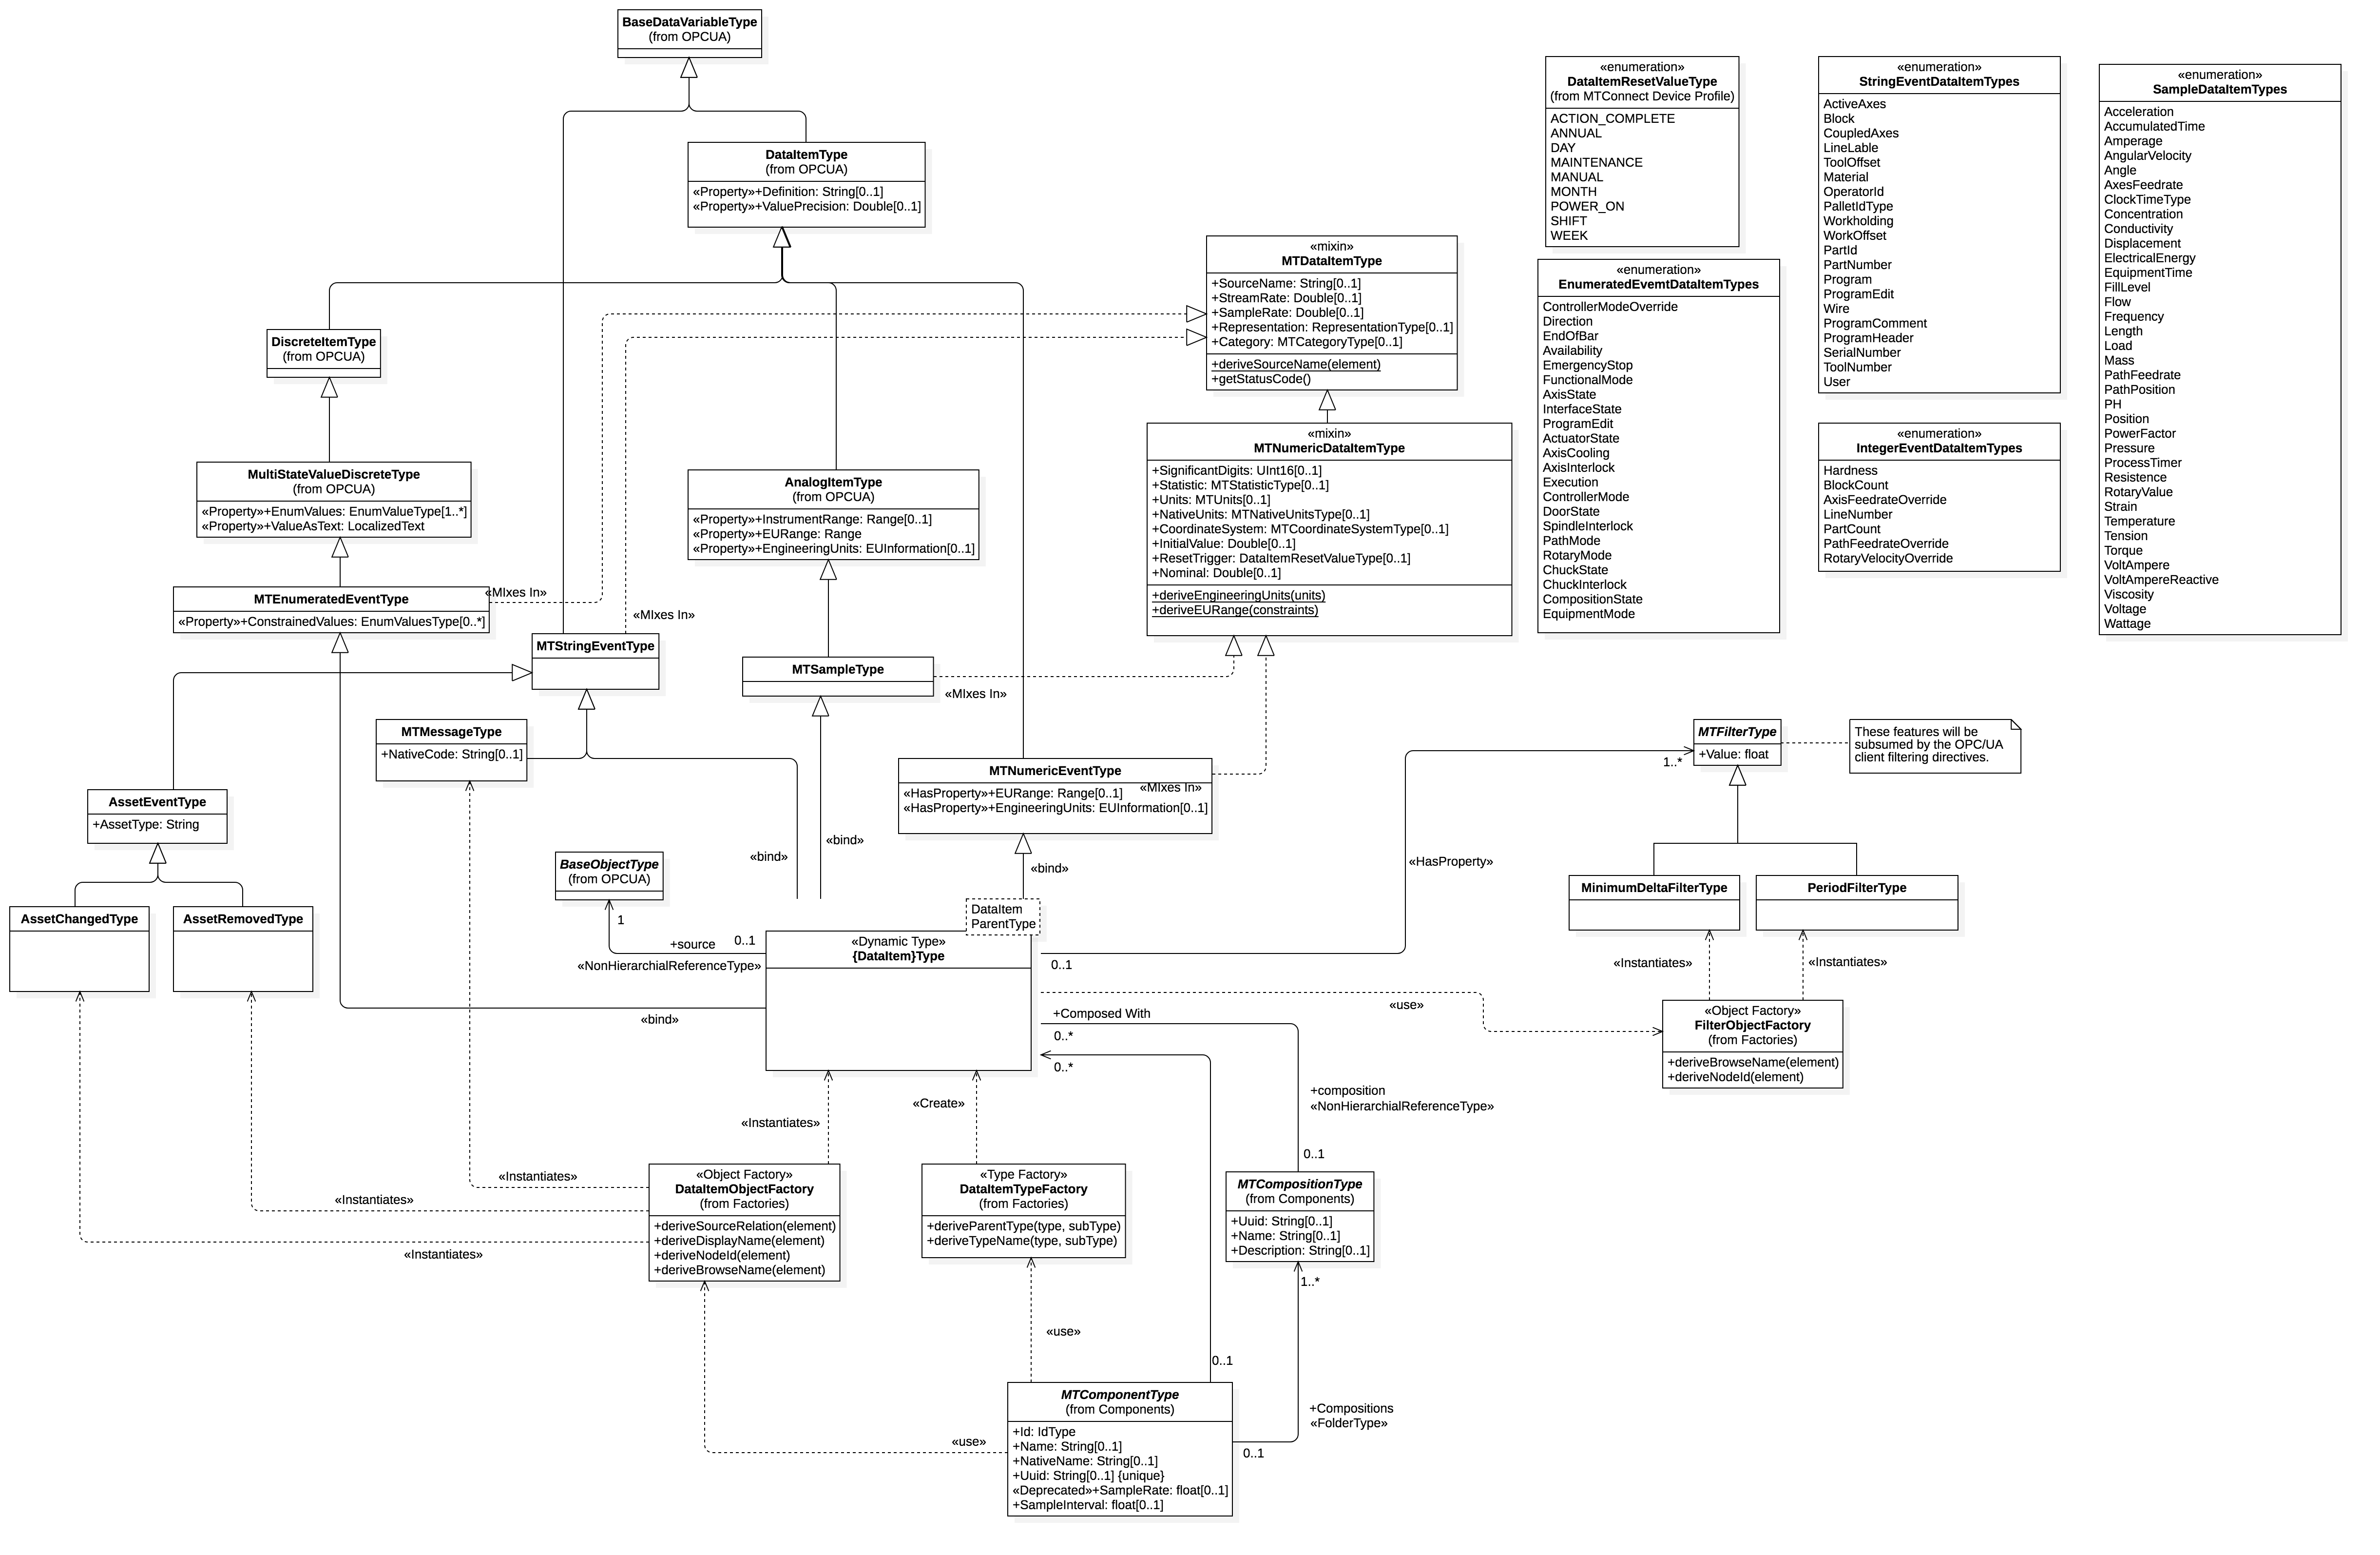
\includegraphics[width=1.0\textwidth]{diagrams/Data Items.png}
  \caption{Data Items Diagram}
  \label{fig:Data Items}
\end{figure}




\subsubsection{Defintion of AssetChangedType} \label{type:AssetChangedType}



Refer to Table \ref{table:AssetChangedType} for detailed definition.

\begin{table}
\centering 
  \caption{AssetChangedType Definition}
  \label{table:AssetChangedType}
\footnotesize
\tabulinesep=3pt
\begin{tabu} to 6in {|X[1.3]|X[1]|X[1.6]|X[2]|X[1.5]|X[1]|} \everyrow{\hline}
\hline
\rowfont\bfseries {Attribute} & \multicolumn{5}{|l|}{Value} \\
\tabucline[1.5pt]{}
BrowseName & \multicolumn{5}{|l|}{AssetChangedType} \\
IsAbstract & \multicolumn{5}{|l|}{False} \\
\tabucline[1.5pt]{}
\rowfont \bfseries References & NodeClass & BrowseName & DataType & TypeDefinition & {Modeling Rule} \\
\multicolumn{6}{|l|}{Subtype of AssetEventType (see section \ref{type:AssetEventType})} \\
\end{tabu}
\end{table} 

\subsubsection{Defintion of AssetEventType} \label{type:AssetEventType}



Refer to Table \ref{table:AssetEventType} for detailed definition.

\begin{table}
\centering 
  \caption{AssetEventType Definition}
  \label{table:AssetEventType}
\footnotesize
\tabulinesep=3pt
\begin{tabu} to 6in {|X[1.3]|X[1]|X[1.6]|X[2]|X[1.5]|X[1]|} \everyrow{\hline}
\hline
\rowfont\bfseries {Attribute} & \multicolumn{5}{|l|}{Value} \\
\tabucline[1.5pt]{}
BrowseName & \multicolumn{5}{|l|}{AssetEventType} \\
IsAbstract & \multicolumn{5}{|l|}{False} \\
\tabucline[1.5pt]{}
\rowfont \bfseries References & NodeClass & BrowseName & DataType & TypeDefinition & {Modeling Rule} \\
\multicolumn{6}{|l|}{Subtype of MTStringEventType (see section \ref{type:MTStringEventType})} \\
HasProperty & Variable & AssetType &  String & PropertyType & Manditory \\
\end{tabu}
\end{table} 

\subsubsection{Defintion of AssetRemovedType} \label{type:AssetRemovedType}



Refer to Table \ref{table:AssetRemovedType} for detailed definition.

\begin{table}
\centering 
  \caption{AssetRemovedType Definition}
  \label{table:AssetRemovedType}
\footnotesize
\tabulinesep=3pt
\begin{tabu} to 6in {|X[1.3]|X[1]|X[1.6]|X[2]|X[1.5]|X[1]|} \everyrow{\hline}
\hline
\rowfont\bfseries {Attribute} & \multicolumn{5}{|l|}{Value} \\
\tabucline[1.5pt]{}
BrowseName & \multicolumn{5}{|l|}{AssetRemovedType} \\
IsAbstract & \multicolumn{5}{|l|}{False} \\
\tabucline[1.5pt]{}
\rowfont \bfseries References & NodeClass & BrowseName & DataType & TypeDefinition & {Modeling Rule} \\
\multicolumn{6}{|l|}{Subtype of AssetEventType (see section \ref{type:AssetEventType})} \\
\end{tabu}
\end{table} 

\subsubsection{Defintion of MTDataItemType} \label{type:MTDataItemType}

The data item mixin will inject the properties and the methods into the related classes. This facility is similar to the Ruby module mixin or the Scala traits.

Refer to Table \ref{table:MTDataItemType} for detailed definition.

\begin{table}
\centering 
  \caption{MTDataItemType Definition}
  \label{table:MTDataItemType}
\footnotesize
\tabulinesep=3pt
\begin{tabu} to 6in {|X[1.3]|X[1]|X[1.6]|X[2]|X[1.5]|X[1]|} \everyrow{\hline}
\hline
\rowfont\bfseries {Attribute} & \multicolumn{5}{|l|}{Value} \\
\tabucline[1.5pt]{}
BrowseName & \multicolumn{5}{|l|}{MTDataItemType} \\
IsAbstract & \multicolumn{5}{|l|}{False} \\
\tabucline[1.5pt]{}
\rowfont \bfseries References & NodeClass & BrowseName & DataType & TypeDefinition & {Modeling Rule} \\
HasProperty & Variable & SourceName &  String & PropertyType & Optional \\
HasProperty & Variable & StreamRate &  Double & PropertyType & Optional \\
HasProperty & Variable & SampleRate &  Double & PropertyType & Optional \\
HasProperty & Variable & Representation &  RepresentationType & PropertyType & Optional \\
HasProperty & Variable & Category &  MTCategoryType & PropertyType & Optional \\
HasProperty & Variable & <Dynamic> &  MTFilterType & <Dynamic> & Optional \\
HasComponent & Object & source &   & BaseObjectType & Optional \\
\end{tabu}
\end{table} 

\subsubsection{Defintion of MTEnumeratedEventType} \label{type:MTEnumeratedEventType}

All Data Items with Category EVENT having a Controlled Vocabularies will be of this type. Otherwise, MTString

Refer to Table \ref{table:MTEnumeratedEventType} for detailed definition.

\begin{table}
\centering 
  \caption{MTEnumeratedEventType Definition}
  \label{table:MTEnumeratedEventType}
\footnotesize
\tabulinesep=3pt
\begin{tabu} to 6in {|X[1.3]|X[1]|X[1.6]|X[2]|X[1.5]|X[1]|} \everyrow{\hline}
\hline
\rowfont\bfseries {Attribute} & \multicolumn{5}{|l|}{Value} \\
\tabucline[1.5pt]{}
BrowseName & \multicolumn{5}{|l|}{MTEnumeratedEventType} \\
IsAbstract & \multicolumn{5}{|l|}{False} \\
\tabucline[1.5pt]{}
\rowfont \bfseries References & NodeClass & BrowseName & DataType & TypeDefinition & {Modeling Rule} \\
\multicolumn{6}{|l|}{Subtype of MultiStateValueDiscreteType (See OPCUA Documentation)} \\
HasProperty & Variable & ConstrainedValues &  EnumValuesType & PropertyType & Manditory \\
\end{tabu}
\end{table} 

\subsubsection{Defintion of MTFilterType} \label{type:MTFilterType}

These features will be subsumed by the OPC/UA client filtering directives.

Refer to Table \ref{table:MTFilterType} for detailed definition.

\begin{table}
\centering 
  \caption{MTFilterType Definition}
  \label{table:MTFilterType}
\footnotesize
\tabulinesep=3pt
\begin{tabu} to 6in {|X[1.3]|X[1]|X[1.6]|X[2]|X[1.5]|X[1]|} \everyrow{\hline}
\hline
\rowfont\bfseries {Attribute} & \multicolumn{5}{|l|}{Value} \\
\tabucline[1.5pt]{}
BrowseName & \multicolumn{5}{|l|}{MTFilterType} \\
IsAbstract & \multicolumn{5}{|l|}{True} \\
\tabucline[1.5pt]{}
\rowfont \bfseries References & NodeClass & BrowseName & DataType & TypeDefinition & {Modeling Rule} \\
HasProperty & Variable & Value &  float & PropertyType & Manditory \\
\end{tabu}
\end{table} 

\subsubsection{Defintion of MTMessageType} \label{type:MTMessageType}



Refer to Table \ref{table:MTMessageType} for detailed definition.

\begin{table}
\centering 
  \caption{MTMessageType Definition}
  \label{table:MTMessageType}
\footnotesize
\tabulinesep=3pt
\begin{tabu} to 6in {|X[1.3]|X[1]|X[1.6]|X[2]|X[1.5]|X[1]|} \everyrow{\hline}
\hline
\rowfont\bfseries {Attribute} & \multicolumn{5}{|l|}{Value} \\
\tabucline[1.5pt]{}
BrowseName & \multicolumn{5}{|l|}{MTMessageType} \\
IsAbstract & \multicolumn{5}{|l|}{False} \\
\tabucline[1.5pt]{}
\rowfont \bfseries References & NodeClass & BrowseName & DataType & TypeDefinition & {Modeling Rule} \\
\multicolumn{6}{|l|}{Subtype of MTStringEventType (see section \ref{type:MTStringEventType})} \\
HasProperty & Variable & NativeCode &  String & PropertyType & Optional \\
\end{tabu}
\end{table} 

\subsubsection{Defintion of MTNumericDataItemType} \label{type:MTNumericDataItemType}

These are the additional attributes that are relevent to numeric data items. The factory will evaluate these values and will set the engineering units and the range associated with the parent entity.

Refer to Table \ref{table:MTNumericDataItemType} for detailed definition.

\begin{table}
\centering 
  \caption{MTNumericDataItemType Definition}
  \label{table:MTNumericDataItemType}
\footnotesize
\tabulinesep=3pt
\begin{tabu} to 6in {|X[1.3]|X[1]|X[1.6]|X[2]|X[1.5]|X[1]|} \everyrow{\hline}
\hline
\rowfont\bfseries {Attribute} & \multicolumn{5}{|l|}{Value} \\
\tabucline[1.5pt]{}
BrowseName & \multicolumn{5}{|l|}{MTNumericDataItemType} \\
IsAbstract & \multicolumn{5}{|l|}{False} \\
\tabucline[1.5pt]{}
\rowfont \bfseries References & NodeClass & BrowseName & DataType & TypeDefinition & {Modeling Rule} \\
\multicolumn{6}{|l|}{Subtype of MTDataItemType (see section \ref{type:MTDataItemType})} \\
HasProperty & Variable & SignificantDigits &  UInt16 & PropertyType & Optional \\
HasProperty & Variable & Statistic &  MTStatisticType & PropertyType & Optional \\
HasProperty & Variable & Units &  MTUnits & PropertyType & Optional \\
HasProperty & Variable & NativeUnits &  MTNativeUnitsType & PropertyType & Optional \\
HasProperty & Variable & CoordinateSystem &  MTCoordinateSystemType & PropertyType & Optional \\
HasProperty & Variable & InitialValue &  Double & PropertyType & Optional \\
HasProperty & Variable & ResetTrigger &  DataItemResetValueType & PropertyType & Optional \\
HasProperty & Variable & Nominal &  Double & PropertyType & Optional \\
\end{tabu}
\end{table} 

\subsubsection{Defintion of MTNumericEventType} \label{type:MTNumericEventType}

All data items with category EVENT and a numeric value.

Refer to Table \ref{table:MTNumericEventType} for detailed definition.

\begin{table}
\centering 
  \caption{MTNumericEventType Definition}
  \label{table:MTNumericEventType}
\footnotesize
\tabulinesep=3pt
\begin{tabu} to 6in {|X[1.3]|X[1]|X[1.6]|X[2]|X[1.5]|X[1]|} \everyrow{\hline}
\hline
\rowfont\bfseries {Attribute} & \multicolumn{5}{|l|}{Value} \\
\tabucline[1.5pt]{}
BrowseName & \multicolumn{5}{|l|}{MTNumericEventType} \\
IsAbstract & \multicolumn{5}{|l|}{False} \\
\tabucline[1.5pt]{}
\rowfont \bfseries References & NodeClass & BrowseName & DataType & TypeDefinition & {Modeling Rule} \\
\multicolumn{6}{|l|}{Subtype of DataItemType (See OPCUA Documentation)} \\
HasProperty & Variable & EURange &  Range & PropertyType & Optional \\
HasProperty & Variable & EngineeringUnits &  EUInformation & PropertyType & Optional \\
\end{tabu}
\end{table} 

\subsubsection{Defintion of MTSampleType} \label{type:MTSampleType}

Data Items with category SAMPLE

Refer to Table \ref{table:MTSampleType} for detailed definition.

\begin{table}
\centering 
  \caption{MTSampleType Definition}
  \label{table:MTSampleType}
\footnotesize
\tabulinesep=3pt
\begin{tabu} to 6in {|X[1.3]|X[1]|X[1.6]|X[2]|X[1.5]|X[1]|} \everyrow{\hline}
\hline
\rowfont\bfseries {Attribute} & \multicolumn{5}{|l|}{Value} \\
\tabucline[1.5pt]{}
BrowseName & \multicolumn{5}{|l|}{MTSampleType} \\
IsAbstract & \multicolumn{5}{|l|}{False} \\
\tabucline[1.5pt]{}
\rowfont \bfseries References & NodeClass & BrowseName & DataType & TypeDefinition & {Modeling Rule} \\
\multicolumn{6}{|l|}{Subtype of AnalogItemType (See OPCUA Documentation)} \\
\end{tabu}
\end{table} 

\subsubsection{Defintion of MTStringEventType} \label{type:MTStringEventType}

All data items with category EVENT where the data is freeform text. The set_data_type constraint derives  makes the data type a string for this type.

Refer to Table \ref{table:MTStringEventType} for detailed definition.

\begin{table}
\centering 
  \caption{MTStringEventType Definition}
  \label{table:MTStringEventType}
\footnotesize
\tabulinesep=3pt
\begin{tabu} to 6in {|X[1.3]|X[1]|X[1.6]|X[2]|X[1.5]|X[1]|} \everyrow{\hline}
\hline
\rowfont\bfseries {Attribute} & \multicolumn{5}{|l|}{Value} \\
\tabucline[1.5pt]{}
BrowseName & \multicolumn{5}{|l|}{MTStringEventType} \\
IsAbstract & \multicolumn{5}{|l|}{False} \\
\tabucline[1.5pt]{}
\rowfont \bfseries References & NodeClass & BrowseName & DataType & TypeDefinition & {Modeling Rule} \\
\multicolumn{6}{|l|}{Subtype of BaseDataVariableType (See OPCUA Documentation)} \\
\end{tabu}
\end{table} 

\subsubsection{Defintion of MinimumDeltaFilterType} \label{type:MinimumDeltaFilterType}



Refer to Table \ref{table:MinimumDeltaFilterType} for detailed definition.

\begin{table}
\centering 
  \caption{MinimumDeltaFilterType Definition}
  \label{table:MinimumDeltaFilterType}
\footnotesize
\tabulinesep=3pt
\begin{tabu} to 6in {|X[1.3]|X[1]|X[1.6]|X[2]|X[1.5]|X[1]|} \everyrow{\hline}
\hline
\rowfont\bfseries {Attribute} & \multicolumn{5}{|l|}{Value} \\
\tabucline[1.5pt]{}
BrowseName & \multicolumn{5}{|l|}{MinimumDeltaFilterType} \\
IsAbstract & \multicolumn{5}{|l|}{False} \\
\tabucline[1.5pt]{}
\rowfont \bfseries References & NodeClass & BrowseName & DataType & TypeDefinition & {Modeling Rule} \\
\multicolumn{6}{|l|}{Subtype of MTFilterType (see section \ref{type:MTFilterType})} \\
\end{tabu}
\end{table} 

\subsubsection{Defintion of PeriodFilterType} \label{type:PeriodFilterType}



Refer to Table \ref{table:PeriodFilterType} for detailed definition.

\begin{table}
\centering 
  \caption{PeriodFilterType Definition}
  \label{table:PeriodFilterType}
\footnotesize
\tabulinesep=3pt
\begin{tabu} to 6in {|X[1.3]|X[1]|X[1.6]|X[2]|X[1.5]|X[1]|} \everyrow{\hline}
\hline
\rowfont\bfseries {Attribute} & \multicolumn{5}{|l|}{Value} \\
\tabucline[1.5pt]{}
BrowseName & \multicolumn{5}{|l|}{PeriodFilterType} \\
IsAbstract & \multicolumn{5}{|l|}{False} \\
\tabucline[1.5pt]{}
\rowfont \bfseries References & NodeClass & BrowseName & DataType & TypeDefinition & {Modeling Rule} \\
\multicolumn{6}{|l|}{Subtype of MTFilterType (see section \ref{type:MTFilterType})} \\
\end{tabu}
\end{table} 

\subsubsection{Defintion of {DataItem}Type} \label{type:{DataItem}Type}

For each DataItem the Sub Type, and the Type will be composed to be the  HasTypeDefinition relationship of the object. The BrowseName will also include the Composition Type if a composition Id is provided.

Refer to Table \ref{table:{DataItem}Type} for detailed definition.

\begin{table}
\centering 
  \caption{{DataItem}Type Definition}
  \label{table:{DataItem}Type}
\footnotesize
\tabulinesep=3pt
\begin{tabu} to 6in {|X[1.3]|X[1]|X[1.6]|X[2]|X[1.5]|X[1]|} \everyrow{\hline}
\hline
\rowfont\bfseries {Attribute} & \multicolumn{5}{|l|}{Value} \\
\tabucline[1.5pt]{}
BrowseName & \multicolumn{5}{|l|}{{DataItem}Type} \\
IsAbstract & \multicolumn{5}{|l|}{False} \\
\tabucline[1.5pt]{}
\rowfont \bfseries References & NodeClass & BrowseName & DataType & TypeDefinition & {Modeling Rule} \\
\multicolumn{6}{|l|}{Subtype of MTNumericEventType (see section \ref{type:MTNumericEventType})} \\
\end{tabu}
\end{table} 

\subsection{Conditions}

\begin{figure}
  \centering
    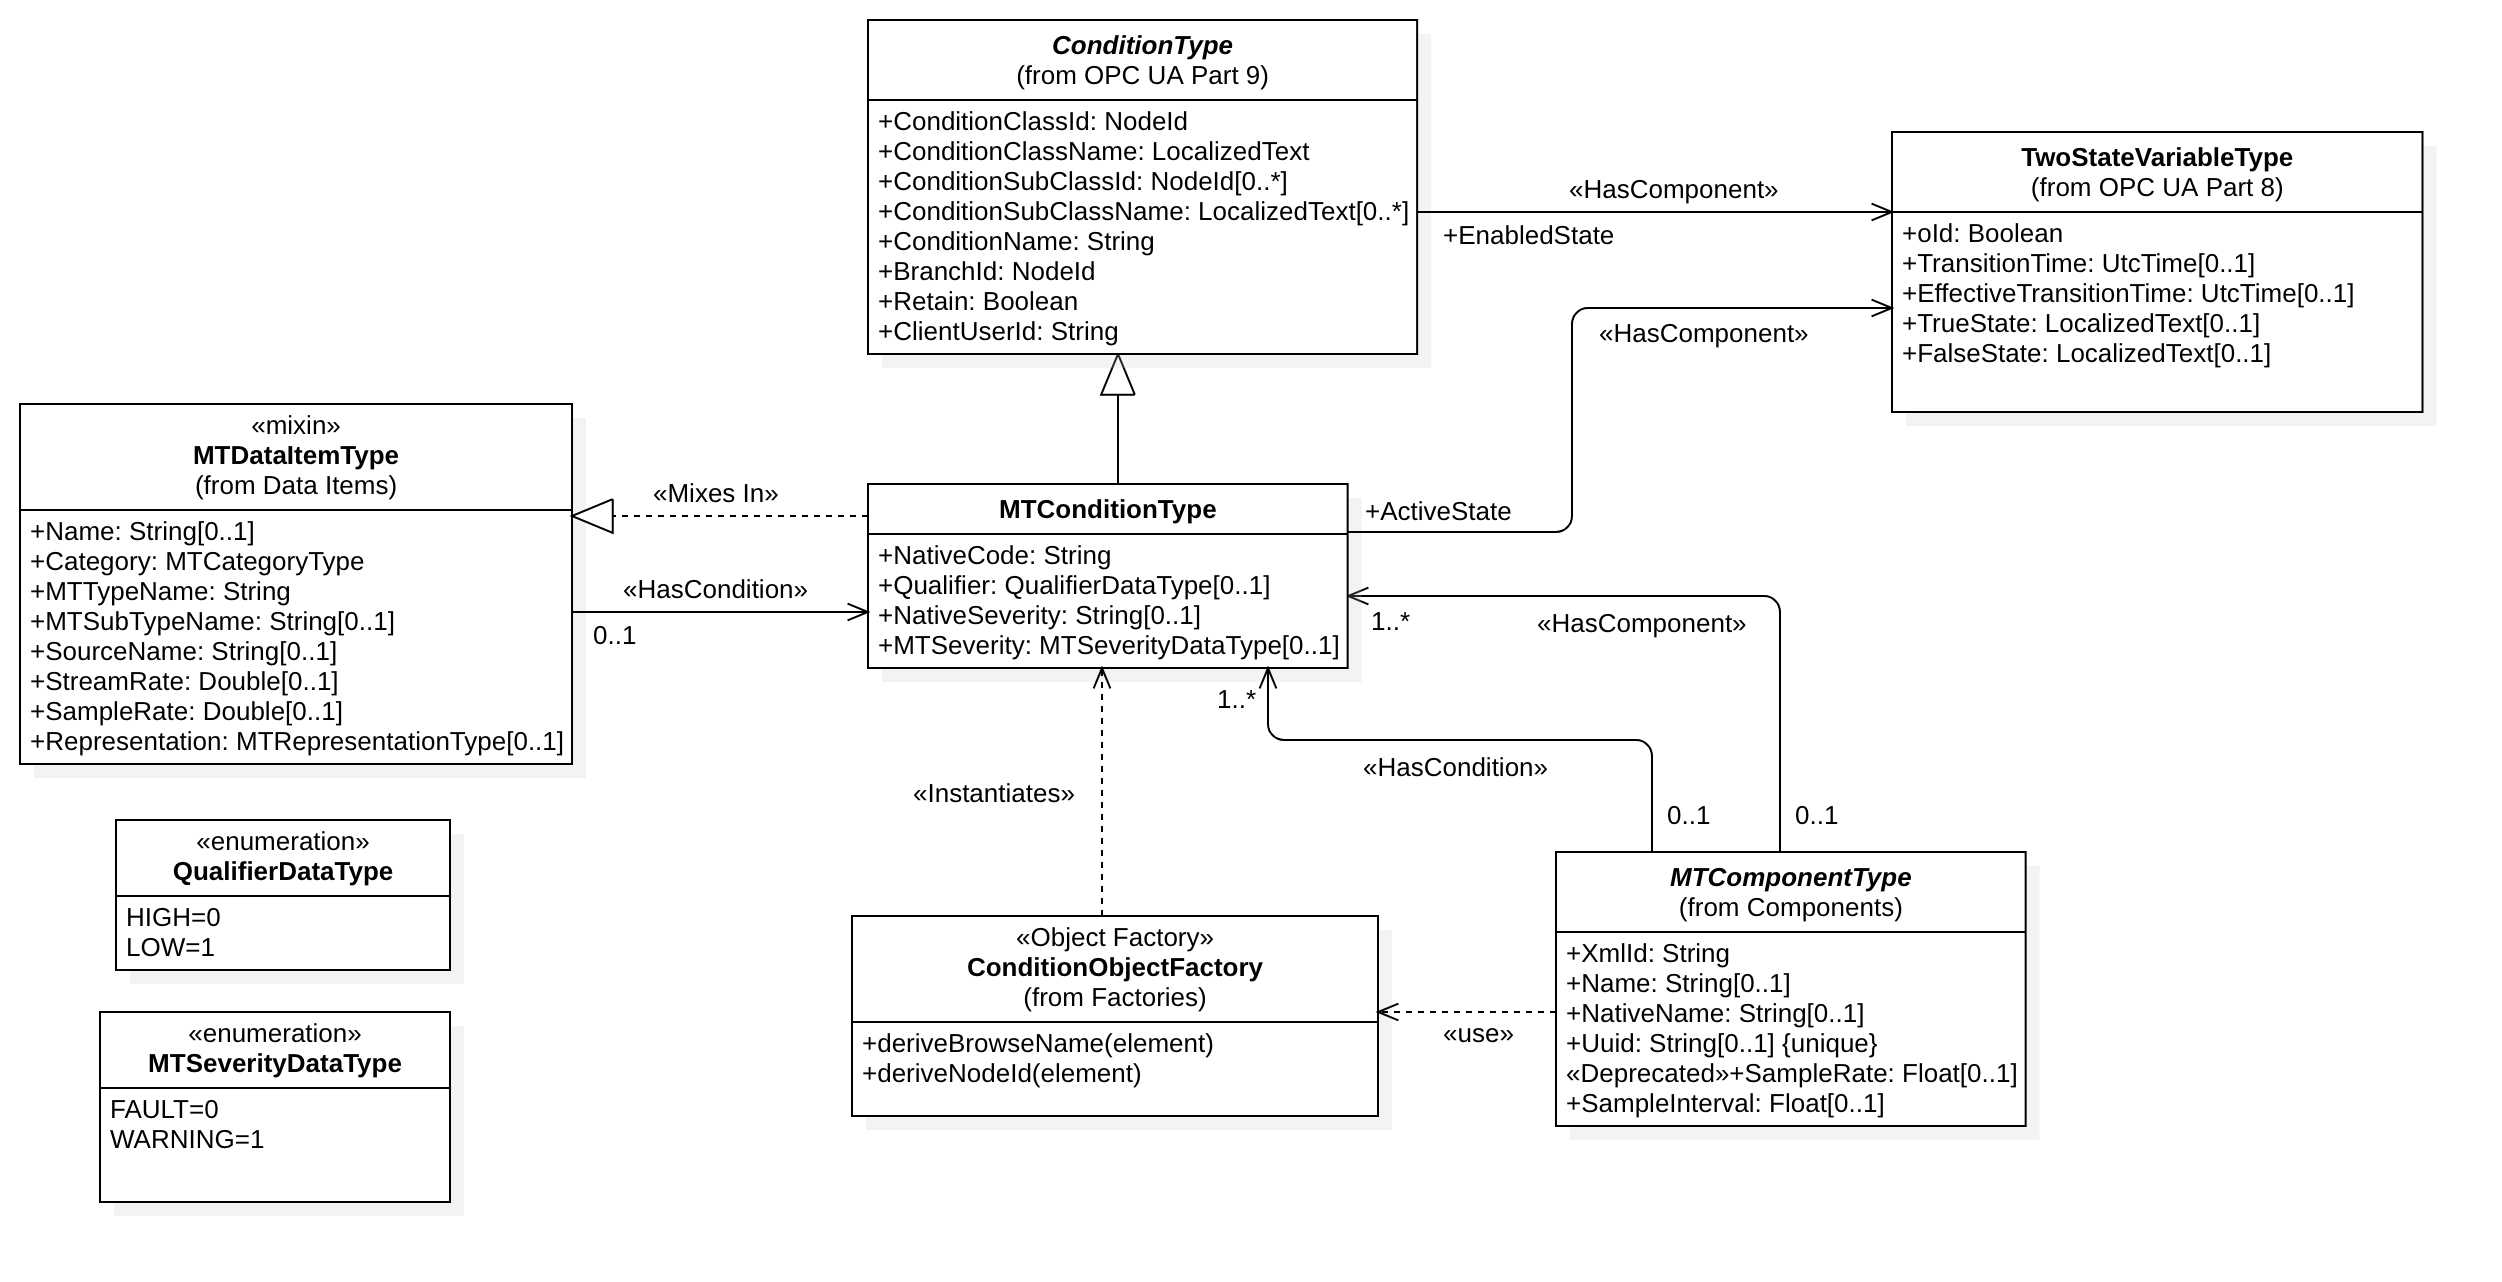
\includegraphics[width=1.0\textwidth]{diagrams/Conditions.png}
  \caption{Conditions Diagram}
  \label{fig:Conditions}
\end{figure}




\subsubsection{Defintion of MTExclusiveLimitConditionType} \label{type:MTExclusiveLimitConditionType}



Refer to Table \ref{table:MTExclusiveLimitConditionType} for detailed definition.

\begin{table}
\centering 
  \caption{MTExclusiveLimitConditionType Definition}
  \label{table:MTExclusiveLimitConditionType}
\footnotesize
\tabulinesep=3pt
\begin{tabu} to 6in {|X[1.3]|X[1]|X[1.6]|X[2]|X[1.5]|X[1]|} \everyrow{\hline}
\hline
\rowfont\bfseries {Attribute} & \multicolumn{5}{|l|}{Value} \\
\tabucline[1.5pt]{}
BrowseName & \multicolumn{5}{|l|}{MTExclusiveLimitConditionType} \\
IsAbstract & \multicolumn{5}{|l|}{False} \\
\tabucline[1.5pt]{}
\rowfont \bfseries References & NodeClass & BrowseName & DataType & TypeDefinition & {Modeling Rule} \\
\multicolumn{6}{|l|}{Subtype of ExclusiveLimitAlarmType (See OPCUA Documentation)} \\
\end{tabu}
\end{table} 

\subsubsection{Defintion of MTNonExclusiveConditionType} \label{type:MTNonExclusiveConditionType}



Refer to Table \ref{table:MTNonExclusiveConditionType} for detailed definition.

\begin{table}
\centering 
  \caption{MTNonExclusiveConditionType Definition}
  \label{table:MTNonExclusiveConditionType}
\footnotesize
\tabulinesep=3pt
\begin{tabu} to 6in {|X[1.3]|X[1]|X[1.6]|X[2]|X[1.5]|X[1]|} \everyrow{\hline}
\hline
\rowfont\bfseries {Attribute} & \multicolumn{5}{|l|}{Value} \\
\tabucline[1.5pt]{}
BrowseName & \multicolumn{5}{|l|}{MTNonExclusiveConditionType} \\
IsAbstract & \multicolumn{5}{|l|}{False} \\
\tabucline[1.5pt]{}
\rowfont \bfseries References & NodeClass & BrowseName & DataType & TypeDefinition & {Modeling Rule} \\
\multicolumn{6}{|l|}{Subtype of NonEclusiveLimitAlarmType (See OPCUA Documentation)} \\
\end{tabu}
\end{table} 

\subsubsection{Defintion of {ConditionClass}Type} \label{type:{ConditionClass}Type}



Refer to Table \ref{table:{ConditionClass}Type} for detailed definition.

\begin{table}
\centering 
  \caption{{ConditionClass}Type Definition}
  \label{table:{ConditionClass}Type}
\footnotesize
\tabulinesep=3pt
\begin{tabu} to 6in {|X[1.3]|X[1]|X[1.6]|X[2]|X[1.5]|X[1]|} \everyrow{\hline}
\hline
\rowfont\bfseries {Attribute} & \multicolumn{5}{|l|}{Value} \\
\tabucline[1.5pt]{}
BrowseName & \multicolumn{5}{|l|}{{ConditionClass}Type} \\
IsAbstract & \multicolumn{5}{|l|}{False} \\
\tabucline[1.5pt]{}
\rowfont \bfseries References & NodeClass & BrowseName & DataType & TypeDefinition & {Modeling Rule} \\
\multicolumn{6}{|l|}{Subtype of SystemConditionClassType (See OPCUA Documentation)} \\
\end{tabu}
\end{table} 

\subsection{Factories}

\begin{figure}
  \centering
    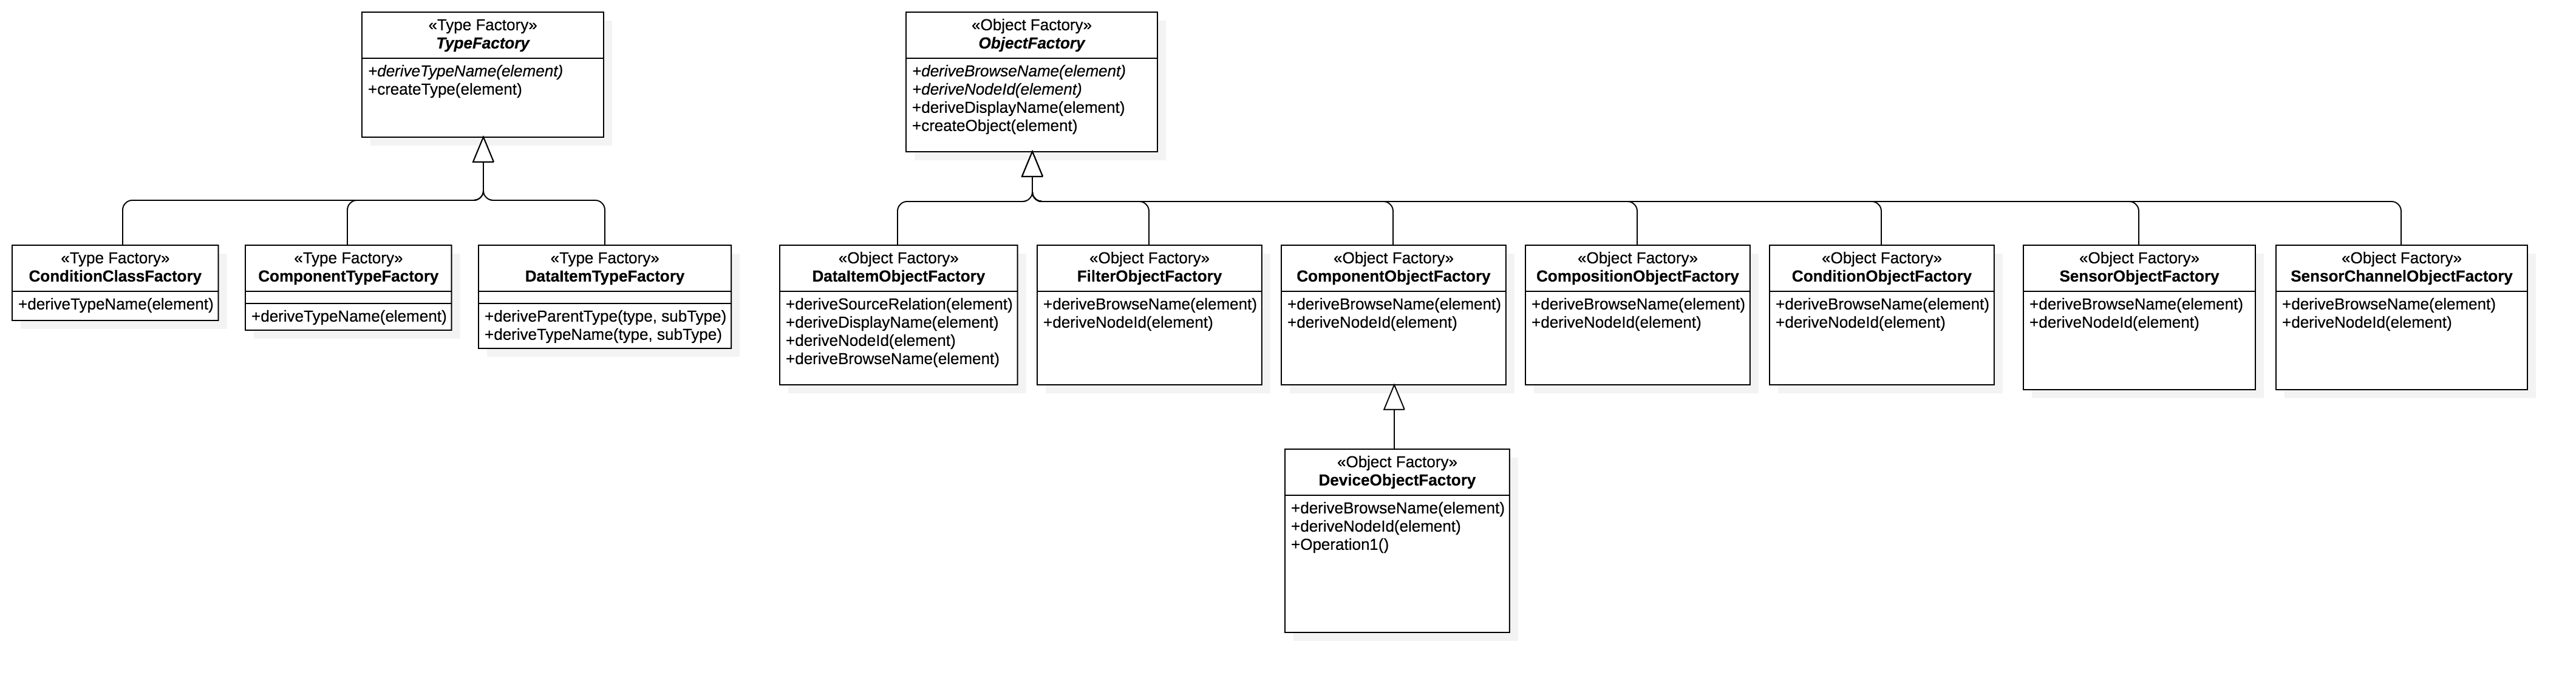
\includegraphics[width=1.0\textwidth]{diagrams/Factories.png}
  \caption{Factories Diagram}
  \label{fig:Factories}
\end{figure}


The factories are not part of the OPC/UA information model. They are a set of helper 
classes that are used to create dynamic types and objects. Since the MTConnect 
information model can be layered on top of the OPC/UA abstrations, the factories
provide the rules for creating the browse and display names for each type.

The factories also create dynamic objects when requried for variables of various
classes when they are required, such as the Data Items and the Components. Some of the
relationships are more complex since they require a dynamic super-type relationship that
relies on the correct placement of the MTConnect elements to be correctly 
represented using the OPC/UA base types.

This is especially evident when mapping the DataItems and the Conditions to the 
MTConnect Information Models and providing sufficent definition to allow for 
unambiguous implementation.

\subsubsection{Defintion of ComponentObjectFactory} \label{type:ComponentObjectFactory}



Refer to Table \ref{table:ComponentObjectFactory} for detailed definition.

\begin{table}
\centering 
  \caption{ComponentObjectFactory Definition}
  \label{table:ComponentObjectFactory}
\footnotesize
\tabulinesep=3pt
\begin{tabu} to 6in {|X[1.3]|X[1]|X[1.6]|X[2]|X[1.5]|X[1]|} \everyrow{\hline}
\hline
\rowfont\bfseries {Attribute} & \multicolumn{5}{|l|}{Value} \\
\tabucline[1.5pt]{}
BrowseName & \multicolumn{5}{|l|}{ComponentObjectFactory} \\
IsAbstract & \multicolumn{5}{|l|}{False} \\
\tabucline[1.5pt]{}
\rowfont \bfseries References & NodeClass & BrowseName & DataType & TypeDefinition & {Modeling Rule} \\
\multicolumn{6}{|l|}{Subtype of ObjectFactory (see section \ref{type:ObjectFactory})} \\
\end{tabu}
\end{table} 

\subsubsection{Defintion of ComponentTypeFactory} \label{type:ComponentTypeFactory}

The `ComponentTypeFactory` creates component types using the MTConnect XML element as an input. 
The factory takes the `QName` (or qualified name) of the XML element and then appends `Type`. For 
example an `<Controller id='...'></...>` element will create an OPC/UA `ControllerType` type definition 
as an extension of the base `MTControllerType`. 

Currently there is no additional abstractions or super types required by the companion specification. 
The types will be a single level where each Component is a sub-type of the base `MTComponentType`.


Refer to Table \ref{table:ComponentTypeFactory} for detailed definition.

\begin{table}
\centering 
  \caption{ComponentTypeFactory Definition}
  \label{table:ComponentTypeFactory}
\footnotesize
\tabulinesep=3pt
\begin{tabu} to 6in {|X[1.3]|X[1]|X[1.6]|X[2]|X[1.5]|X[1]|} \everyrow{\hline}
\hline
\rowfont\bfseries {Attribute} & \multicolumn{5}{|l|}{Value} \\
\tabucline[1.5pt]{}
BrowseName & \multicolumn{5}{|l|}{ComponentTypeFactory} \\
IsAbstract & \multicolumn{5}{|l|}{False} \\
\tabucline[1.5pt]{}
\rowfont \bfseries References & NodeClass & BrowseName & DataType & TypeDefinition & {Modeling Rule} \\
\multicolumn{6}{|l|}{Subtype of TypeFactory (see section \ref{type:TypeFactory})} \\
\end{tabu}
\end{table} 

\subsubsection{Defintion of CompositionObjectFactory} \label{type:CompositionObjectFactory}



Refer to Table \ref{table:CompositionObjectFactory} for detailed definition.

\begin{table}
\centering 
  \caption{CompositionObjectFactory Definition}
  \label{table:CompositionObjectFactory}
\footnotesize
\tabulinesep=3pt
\begin{tabu} to 6in {|X[1.3]|X[1]|X[1.6]|X[2]|X[1.5]|X[1]|} \everyrow{\hline}
\hline
\rowfont\bfseries {Attribute} & \multicolumn{5}{|l|}{Value} \\
\tabucline[1.5pt]{}
BrowseName & \multicolumn{5}{|l|}{CompositionObjectFactory} \\
IsAbstract & \multicolumn{5}{|l|}{False} \\
\tabucline[1.5pt]{}
\rowfont \bfseries References & NodeClass & BrowseName & DataType & TypeDefinition & {Modeling Rule} \\
\multicolumn{6}{|l|}{Subtype of ObjectFactory (see section \ref{type:ObjectFactory})} \\
\end{tabu}
\end{table} 

\subsubsection{Defintion of CompositionTypeFactory} \label{type:CompositionTypeFactory}



Refer to Table \ref{table:CompositionTypeFactory} for detailed definition.

\begin{table}
\centering 
  \caption{CompositionTypeFactory Definition}
  \label{table:CompositionTypeFactory}
\footnotesize
\tabulinesep=3pt
\begin{tabu} to 6in {|X[1.3]|X[1]|X[1.6]|X[2]|X[1.5]|X[1]|} \everyrow{\hline}
\hline
\rowfont\bfseries {Attribute} & \multicolumn{5}{|l|}{Value} \\
\tabucline[1.5pt]{}
BrowseName & \multicolumn{5}{|l|}{CompositionTypeFactory} \\
IsAbstract & \multicolumn{5}{|l|}{False} \\
\tabucline[1.5pt]{}
\rowfont \bfseries References & NodeClass & BrowseName & DataType & TypeDefinition & {Modeling Rule} \\
\end{tabu}
\end{table} 

\subsubsection{Defintion of ConditionClassFactory} \label{type:ConditionClassFactory}



Refer to Table \ref{table:ConditionClassFactory} for detailed definition.

\begin{table}
\centering 
  \caption{ConditionClassFactory Definition}
  \label{table:ConditionClassFactory}
\footnotesize
\tabulinesep=3pt
\begin{tabu} to 6in {|X[1.3]|X[1]|X[1.6]|X[2]|X[1.5]|X[1]|} \everyrow{\hline}
\hline
\rowfont\bfseries {Attribute} & \multicolumn{5}{|l|}{Value} \\
\tabucline[1.5pt]{}
BrowseName & \multicolumn{5}{|l|}{ConditionClassFactory} \\
IsAbstract & \multicolumn{5}{|l|}{False} \\
\tabucline[1.5pt]{}
\rowfont \bfseries References & NodeClass & BrowseName & DataType & TypeDefinition & {Modeling Rule} \\
\multicolumn{6}{|l|}{Subtype of TypeFactory (see section \ref{type:TypeFactory})} \\
\end{tabu}
\end{table} 

\subsubsection{Defintion of ConditionObjectFactory} \label{type:ConditionObjectFactory}



Refer to Table \ref{table:ConditionObjectFactory} for detailed definition.

\begin{table}
\centering 
  \caption{ConditionObjectFactory Definition}
  \label{table:ConditionObjectFactory}
\footnotesize
\tabulinesep=3pt
\begin{tabu} to 6in {|X[1.3]|X[1]|X[1.6]|X[2]|X[1.5]|X[1]|} \everyrow{\hline}
\hline
\rowfont\bfseries {Attribute} & \multicolumn{5}{|l|}{Value} \\
\tabucline[1.5pt]{}
BrowseName & \multicolumn{5}{|l|}{ConditionObjectFactory} \\
IsAbstract & \multicolumn{5}{|l|}{False} \\
\tabucline[1.5pt]{}
\rowfont \bfseries References & NodeClass & BrowseName & DataType & TypeDefinition & {Modeling Rule} \\
\multicolumn{6}{|l|}{Subtype of ObjectFactory (see section \ref{type:ObjectFactory})} \\
\end{tabu}
\end{table} 

\subsubsection{Defintion of DataItemObjectFactory} \label{type:DataItemObjectFactory}



Refer to Table \ref{table:DataItemObjectFactory} for detailed definition.

\begin{table}
\centering 
  \caption{DataItemObjectFactory Definition}
  \label{table:DataItemObjectFactory}
\footnotesize
\tabulinesep=3pt
\begin{tabu} to 6in {|X[1.3]|X[1]|X[1.6]|X[2]|X[1.5]|X[1]|} \everyrow{\hline}
\hline
\rowfont\bfseries {Attribute} & \multicolumn{5}{|l|}{Value} \\
\tabucline[1.5pt]{}
BrowseName & \multicolumn{5}{|l|}{DataItemObjectFactory} \\
IsAbstract & \multicolumn{5}{|l|}{False} \\
\tabucline[1.5pt]{}
\rowfont \bfseries References & NodeClass & BrowseName & DataType & TypeDefinition & {Modeling Rule} \\
\multicolumn{6}{|l|}{Subtype of ObjectFactory (see section \ref{type:ObjectFactory})} \\
\end{tabu}
\end{table} 

\subsubsection{Defintion of DataItemTypeFactory} \label{type:DataItemTypeFactory}

Based on the data item category, type, and subType, this class creates a new OPC/UA type and also provides the template parameter for the ParentType from which this type is derived. 

See the Data Item Type Factory.

Refer to Table \ref{table:DataItemTypeFactory} for detailed definition.

\begin{table}
\centering 
  \caption{DataItemTypeFactory Definition}
  \label{table:DataItemTypeFactory}
\footnotesize
\tabulinesep=3pt
\begin{tabu} to 6in {|X[1.3]|X[1]|X[1.6]|X[2]|X[1.5]|X[1]|} \everyrow{\hline}
\hline
\rowfont\bfseries {Attribute} & \multicolumn{5}{|l|}{Value} \\
\tabucline[1.5pt]{}
BrowseName & \multicolumn{5}{|l|}{DataItemTypeFactory} \\
IsAbstract & \multicolumn{5}{|l|}{False} \\
\tabucline[1.5pt]{}
\rowfont \bfseries References & NodeClass & BrowseName & DataType & TypeDefinition & {Modeling Rule} \\
\multicolumn{6}{|l|}{Subtype of TypeFactory (see section \ref{type:TypeFactory})} \\
\end{tabu}
\end{table} 

\subsubsection{Defintion of DeviceObjectFactory} \label{type:DeviceObjectFactory}

The model instantiation for MTConnect begins with the `Device` MTConnect element and then recursively traverses the sub-elements. The device will the capabilities in the component factory to generate all the data items and component types. 

Refer to Table \ref{table:DeviceObjectFactory} for detailed definition.

\begin{table}
\centering 
  \caption{DeviceObjectFactory Definition}
  \label{table:DeviceObjectFactory}
\footnotesize
\tabulinesep=3pt
\begin{tabu} to 6in {|X[1.3]|X[1]|X[1.6]|X[2]|X[1.5]|X[1]|} \everyrow{\hline}
\hline
\rowfont\bfseries {Attribute} & \multicolumn{5}{|l|}{Value} \\
\tabucline[1.5pt]{}
BrowseName & \multicolumn{5}{|l|}{DeviceObjectFactory} \\
IsAbstract & \multicolumn{5}{|l|}{False} \\
\tabucline[1.5pt]{}
\rowfont \bfseries References & NodeClass & BrowseName & DataType & TypeDefinition & {Modeling Rule} \\
\multicolumn{6}{|l|}{Subtype of ComponentObjectFactory (see section \ref{type:ComponentObjectFactory})} \\
\end{tabu}
\end{table} 

\subsubsection{Defintion of FilterObjectFactory} \label{type:FilterObjectFactory}

Creates filters based on the type attribute of the Filter element. 

Refer to Table \ref{table:FilterObjectFactory} for detailed definition.

\begin{table}
\centering 
  \caption{FilterObjectFactory Definition}
  \label{table:FilterObjectFactory}
\footnotesize
\tabulinesep=3pt
\begin{tabu} to 6in {|X[1.3]|X[1]|X[1.6]|X[2]|X[1.5]|X[1]|} \everyrow{\hline}
\hline
\rowfont\bfseries {Attribute} & \multicolumn{5}{|l|}{Value} \\
\tabucline[1.5pt]{}
BrowseName & \multicolumn{5}{|l|}{FilterObjectFactory} \\
IsAbstract & \multicolumn{5}{|l|}{False} \\
\tabucline[1.5pt]{}
\rowfont \bfseries References & NodeClass & BrowseName & DataType & TypeDefinition & {Modeling Rule} \\
\multicolumn{6}{|l|}{Subtype of ObjectFactory (see section \ref{type:ObjectFactory})} \\
\end{tabu}
\end{table} 

\subsubsection{Defintion of ObjectFactory} \label{type:ObjectFactory}



Refer to Table \ref{table:ObjectFactory} for detailed definition.

\begin{table}
\centering 
  \caption{ObjectFactory Definition}
  \label{table:ObjectFactory}
\footnotesize
\tabulinesep=3pt
\begin{tabu} to 6in {|X[1.3]|X[1]|X[1.6]|X[2]|X[1.5]|X[1]|} \everyrow{\hline}
\hline
\rowfont\bfseries {Attribute} & \multicolumn{5}{|l|}{Value} \\
\tabucline[1.5pt]{}
BrowseName & \multicolumn{5}{|l|}{ObjectFactory} \\
IsAbstract & \multicolumn{5}{|l|}{True} \\
\tabucline[1.5pt]{}
\rowfont \bfseries References & NodeClass & BrowseName & DataType & TypeDefinition & {Modeling Rule} \\
\end{tabu}
\end{table} 

\subsubsection{Defintion of SensorChannelObjectFactory} \label{type:SensorChannelObjectFactory}



Refer to Table \ref{table:SensorChannelObjectFactory} for detailed definition.

\begin{table}
\centering 
  \caption{SensorChannelObjectFactory Definition}
  \label{table:SensorChannelObjectFactory}
\footnotesize
\tabulinesep=3pt
\begin{tabu} to 6in {|X[1.3]|X[1]|X[1.6]|X[2]|X[1.5]|X[1]|} \everyrow{\hline}
\hline
\rowfont\bfseries {Attribute} & \multicolumn{5}{|l|}{Value} \\
\tabucline[1.5pt]{}
BrowseName & \multicolumn{5}{|l|}{SensorChannelObjectFactory} \\
IsAbstract & \multicolumn{5}{|l|}{False} \\
\tabucline[1.5pt]{}
\rowfont \bfseries References & NodeClass & BrowseName & DataType & TypeDefinition & {Modeling Rule} \\
\multicolumn{6}{|l|}{Subtype of ObjectFactory (see section \ref{type:ObjectFactory})} \\
\end{tabu}
\end{table} 

\subsubsection{Defintion of SensorObjectFactory} \label{type:SensorObjectFactory}



Refer to Table \ref{table:SensorObjectFactory} for detailed definition.

\begin{table}
\centering 
  \caption{SensorObjectFactory Definition}
  \label{table:SensorObjectFactory}
\footnotesize
\tabulinesep=3pt
\begin{tabu} to 6in {|X[1.3]|X[1]|X[1.6]|X[2]|X[1.5]|X[1]|} \everyrow{\hline}
\hline
\rowfont\bfseries {Attribute} & \multicolumn{5}{|l|}{Value} \\
\tabucline[1.5pt]{}
BrowseName & \multicolumn{5}{|l|}{SensorObjectFactory} \\
IsAbstract & \multicolumn{5}{|l|}{False} \\
\tabucline[1.5pt]{}
\rowfont \bfseries References & NodeClass & BrowseName & DataType & TypeDefinition & {Modeling Rule} \\
\multicolumn{6}{|l|}{Subtype of ObjectFactory (see section \ref{type:ObjectFactory})} \\
\end{tabu}
\end{table} 

\subsubsection{Defintion of TypeFactory} \label{type:TypeFactory}



Refer to Table \ref{table:TypeFactory} for detailed definition.

\begin{table}
\centering 
  \caption{TypeFactory Definition}
  \label{table:TypeFactory}
\footnotesize
\tabulinesep=3pt
\begin{tabu} to 6in {|X[1.3]|X[1]|X[1.6]|X[2]|X[1.5]|X[1]|} \everyrow{\hline}
\hline
\rowfont\bfseries {Attribute} & \multicolumn{5}{|l|}{Value} \\
\tabucline[1.5pt]{}
BrowseName & \multicolumn{5}{|l|}{TypeFactory} \\
IsAbstract & \multicolumn{5}{|l|}{True} \\
\tabucline[1.5pt]{}
\rowfont \bfseries References & NodeClass & BrowseName & DataType & TypeDefinition & {Modeling Rule} \\
\end{tabu}
\end{table} 

\subsection{MTConnect Device Profile}

\begin{figure}
  \centering
    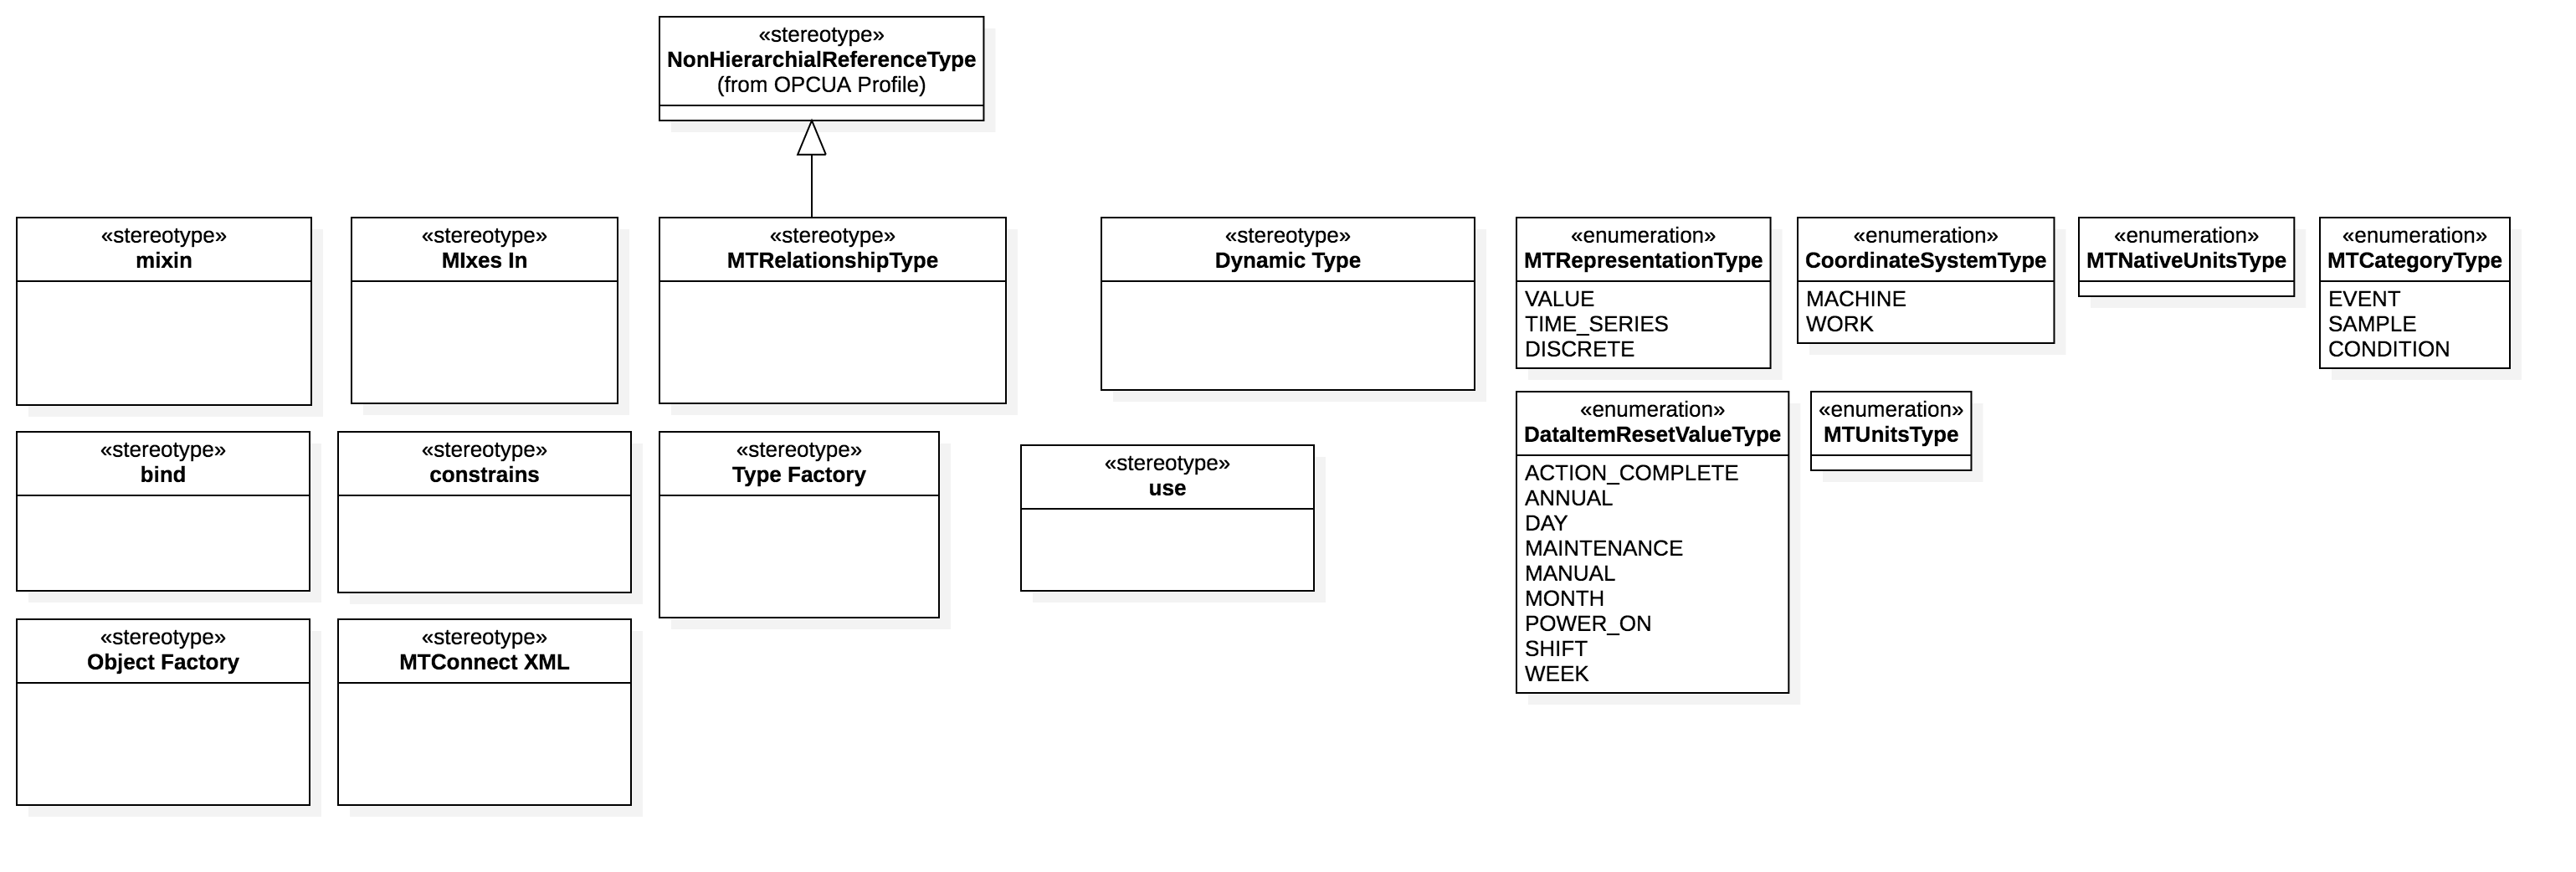
\includegraphics[width=1.0\textwidth]{diagrams/MTConnect Device Profile.png}
  \caption{MTConnect Device Profile Diagram}
  \label{fig:MTConnect Device Profile}
\end{figure}


The device profile documents the common data types and stereotypes that are 
used to construct the model. A stereotype is a design or modeling pattern that 
provides additional information about the type or the relationship between types. 

It can also identify the behavior of a property or the role the type or relation
will play in the model. 

Stereotypes are used throughout the model to provide additional information that 
will halp provide context and definition to aid in better understanding the
data model.

\subsubsection{Defintion of Dynamic Type} \label{type:Dynamic Type}



Refer to Table \ref{table:Dynamic Type} for detailed definition.

\begin{table}
\centering 
  \caption{Dynamic Type Definition}
  \label{table:Dynamic Type}
\footnotesize
\tabulinesep=3pt
\begin{tabu} to 6in {|X[1.3]|X[1]|X[1.6]|X[2]|X[1.5]|X[1]|} \everyrow{\hline}
\hline
\rowfont\bfseries {Attribute} & \multicolumn{5}{|l|}{Value} \\
\tabucline[1.5pt]{}
BrowseName & \multicolumn{5}{|l|}{Dynamic Type} \\
IsAbstract & \multicolumn{5}{|l|}{False} \\
\tabucline[1.5pt]{}
\rowfont \bfseries References & NodeClass & BrowseName & DataType & TypeDefinition & {Modeling Rule} \\
\end{tabu}
\end{table} 

\subsubsection{Defintion of MIxes In} \label{type:MIxes In}



Refer to Table \ref{table:MIxes In} for detailed definition.

\begin{table}
\centering 
  \caption{MIxes In Definition}
  \label{table:MIxes In}
\footnotesize
\tabulinesep=3pt
\begin{tabu} to 6in {|X[1.3]|X[1]|X[1.6]|X[2]|X[1.5]|X[1]|} \everyrow{\hline}
\hline
\rowfont\bfseries {Attribute} & \multicolumn{5}{|l|}{Value} \\
\tabucline[1.5pt]{}
BrowseName & \multicolumn{5}{|l|}{MIxes In} \\
IsAbstract & \multicolumn{5}{|l|}{False} \\
\tabucline[1.5pt]{}
\rowfont \bfseries References & NodeClass & BrowseName & DataType & TypeDefinition & {Modeling Rule} \\
\end{tabu}
\end{table} 

\subsubsection{Defintion of MTConnect XML} \label{type:MTConnect XML}



Refer to Table \ref{table:MTConnect XML} for detailed definition.

\begin{table}
\centering 
  \caption{MTConnect XML Definition}
  \label{table:MTConnect XML}
\footnotesize
\tabulinesep=3pt
\begin{tabu} to 6in {|X[1.3]|X[1]|X[1.6]|X[2]|X[1.5]|X[1]|} \everyrow{\hline}
\hline
\rowfont\bfseries {Attribute} & \multicolumn{5}{|l|}{Value} \\
\tabucline[1.5pt]{}
BrowseName & \multicolumn{5}{|l|}{MTConnect XML} \\
IsAbstract & \multicolumn{5}{|l|}{False} \\
\tabucline[1.5pt]{}
\rowfont \bfseries References & NodeClass & BrowseName & DataType & TypeDefinition & {Modeling Rule} \\
\end{tabu}
\end{table} 

\subsubsection{Defintion of MTRelationshipType} \label{type:MTRelationshipType}



Refer to Table \ref{table:MTRelationshipType} for detailed definition.

\begin{table}
\centering 
  \caption{MTRelationshipType Definition}
  \label{table:MTRelationshipType}
\footnotesize
\tabulinesep=3pt
\begin{tabu} to 6in {|X[1.3]|X[1]|X[1.6]|X[2]|X[1.5]|X[1]|} \everyrow{\hline}
\hline
\rowfont\bfseries {Attribute} & \multicolumn{5}{|l|}{Value} \\
\tabucline[1.5pt]{}
BrowseName & \multicolumn{5}{|l|}{MTRelationshipType} \\
IsAbstract & \multicolumn{5}{|l|}{False} \\
\tabucline[1.5pt]{}
\rowfont \bfseries References & NodeClass & BrowseName & DataType & TypeDefinition & {Modeling Rule} \\
\multicolumn{6}{|l|}{Subtype of NonHierarchialReferenceType (See OPCUA Profile Documentation)} \\
\end{tabu}
\end{table} 

\subsubsection{Defintion of Object Factory} \label{type:Object Factory}



Refer to Table \ref{table:Object Factory} for detailed definition.

\begin{table}
\centering 
  \caption{Object Factory Definition}
  \label{table:Object Factory}
\footnotesize
\tabulinesep=3pt
\begin{tabu} to 6in {|X[1.3]|X[1]|X[1.6]|X[2]|X[1.5]|X[1]|} \everyrow{\hline}
\hline
\rowfont\bfseries {Attribute} & \multicolumn{5}{|l|}{Value} \\
\tabucline[1.5pt]{}
BrowseName & \multicolumn{5}{|l|}{Object Factory} \\
IsAbstract & \multicolumn{5}{|l|}{False} \\
\tabucline[1.5pt]{}
\rowfont \bfseries References & NodeClass & BrowseName & DataType & TypeDefinition & {Modeling Rule} \\
\end{tabu}
\end{table} 

\subsubsection{Defintion of Type Factory} \label{type:Type Factory}



Refer to Table \ref{table:Type Factory} for detailed definition.

\begin{table}
\centering 
  \caption{Type Factory Definition}
  \label{table:Type Factory}
\footnotesize
\tabulinesep=3pt
\begin{tabu} to 6in {|X[1.3]|X[1]|X[1.6]|X[2]|X[1.5]|X[1]|} \everyrow{\hline}
\hline
\rowfont\bfseries {Attribute} & \multicolumn{5}{|l|}{Value} \\
\tabucline[1.5pt]{}
BrowseName & \multicolumn{5}{|l|}{Type Factory} \\
IsAbstract & \multicolumn{5}{|l|}{False} \\
\tabucline[1.5pt]{}
\rowfont \bfseries References & NodeClass & BrowseName & DataType & TypeDefinition & {Modeling Rule} \\
\end{tabu}
\end{table} 

\subsubsection{Defintion of bind} \label{type:bind}



Refer to Table \ref{table:bind} for detailed definition.

\begin{table}
\centering 
  \caption{bind Definition}
  \label{table:bind}
\footnotesize
\tabulinesep=3pt
\begin{tabu} to 6in {|X[1.3]|X[1]|X[1.6]|X[2]|X[1.5]|X[1]|} \everyrow{\hline}
\hline
\rowfont\bfseries {Attribute} & \multicolumn{5}{|l|}{Value} \\
\tabucline[1.5pt]{}
BrowseName & \multicolumn{5}{|l|}{bind} \\
IsAbstract & \multicolumn{5}{|l|}{False} \\
\tabucline[1.5pt]{}
\rowfont \bfseries References & NodeClass & BrowseName & DataType & TypeDefinition & {Modeling Rule} \\
\end{tabu}
\end{table} 

\subsubsection{Defintion of constrains} \label{type:constrains}



Refer to Table \ref{table:constrains} for detailed definition.

\begin{table}
\centering 
  \caption{constrains Definition}
  \label{table:constrains}
\footnotesize
\tabulinesep=3pt
\begin{tabu} to 6in {|X[1.3]|X[1]|X[1.6]|X[2]|X[1.5]|X[1]|} \everyrow{\hline}
\hline
\rowfont\bfseries {Attribute} & \multicolumn{5}{|l|}{Value} \\
\tabucline[1.5pt]{}
BrowseName & \multicolumn{5}{|l|}{constrains} \\
IsAbstract & \multicolumn{5}{|l|}{False} \\
\tabucline[1.5pt]{}
\rowfont \bfseries References & NodeClass & BrowseName & DataType & TypeDefinition & {Modeling Rule} \\
\end{tabu}
\end{table} 

\subsubsection{Defintion of mixin} \label{type:mixin}

The contents properties and the behavior of the class are combined with another class.

Refer to Table \ref{table:mixin} for detailed definition.

\begin{table}
\centering 
  \caption{mixin Definition}
  \label{table:mixin}
\footnotesize
\tabulinesep=3pt
\begin{tabu} to 6in {|X[1.3]|X[1]|X[1.6]|X[2]|X[1.5]|X[1]|} \everyrow{\hline}
\hline
\rowfont\bfseries {Attribute} & \multicolumn{5}{|l|}{Value} \\
\tabucline[1.5pt]{}
BrowseName & \multicolumn{5}{|l|}{mixin} \\
IsAbstract & \multicolumn{5}{|l|}{False} \\
\tabucline[1.5pt]{}
\rowfont \bfseries References & NodeClass & BrowseName & DataType & TypeDefinition & {Modeling Rule} \\
\end{tabu}
\end{table} 

\subsubsection{Defintion of use} \label{type:use}

The use stereotype indicates that one class uses as a helper to perform 
a specific operation or activity. This stereotype is mainly used to indicate
that a specific factory is being employed by another type to create dynamic
properties or relationships.

Refer to Table \ref{table:use} for detailed definition.

\begin{table}
\centering 
  \caption{use Definition}
  \label{table:use}
\footnotesize
\tabulinesep=3pt
\begin{tabu} to 6in {|X[1.3]|X[1]|X[1.6]|X[2]|X[1.5]|X[1]|} \everyrow{\hline}
\hline
\rowfont\bfseries {Attribute} & \multicolumn{5}{|l|}{Value} \\
\tabucline[1.5pt]{}
BrowseName & \multicolumn{5}{|l|}{use} \\
IsAbstract & \multicolumn{5}{|l|}{False} \\
\tabucline[1.5pt]{}
\rowfont \bfseries References & NodeClass & BrowseName & DataType & TypeDefinition & {Modeling Rule} \\
\end{tabu}
\end{table} 

